\documentclass{article}
\usepackage{fullpage}
\usepackage{amsmath,amssymb}
\usepackage{amsthm}
\usepackage{graphicx}
\usepackage{natbib}
\usepackage[colorlinks=false]{hyperref}
\usepackage{bm}
\usepackage{todonotes}

\newcommand{\peter}[1]{\todo[color=green!40]{Peter: #1}}
\newcommand{\erick}[1]{\todo[color=purple!40]{Erick: #1}}

\newcommand{\E}{\mathbb{E}}
\renewcommand{\P}{\mathbb{P}}
\newcommand{\calS}{\mathcal{S}}  % set of states
\newcommand{\calT}{\mathcal{T}}  % set of transition triples
\newcommand{\nA}{\mbox{A}}  % nucleotides:
\newcommand{\nC}{\mbox{C}}
\newcommand{\nG}{\mbox{G}}
\newcommand{\nT}{\mbox{T}}
\newcommand{\join}{\oplus}  % matches
\newcommand{\st}{\colon}  % such that
\newcommand{\var}{\mathop{\mbox{var}}}
\newcommand{\cov}{\mathop{\mbox{cov}}}
\newcommand{\given}{\;\mid\;}
\newcommand{\like}{\mathcal L}
\newcommand{\loglike}{\ell}
\newcommand{\alike}{\widetilde{\like}}
\newcommand{\aloglike}{\widetilde{\loglike}}

\theoremstyle{plain}
\newtheorem{theorem}{Theorem}
\theoremstyle{definition}
\newtheorem{example}{Example}[section]

\bibliographystyle{plainnat}

\begin{document}

\title{Inference using context-dependent models of mutation}
\author{}

\maketitle

\begin{abstract}
\end{abstract}

\section*{Introduction}

It not uncommon to encounter models
consisting of a lattice of sites,
each site taking one of a finite collection of possible states,
and whose stochastic, temporal evolution is Markov and governed by a set of local rules.
For instance, at each site may sit
a nucelotide whose mutation rate depends on physical properties determined by the nearby DNA sequence;
a cell whose infection status depends on the state of its neighbors;
or a particle whose spin is perturbed by external noise to a state whose distribution depends on the local energy configuration.
Practical use of such models often requires
inferring transition rules
based on observations of the system at several time points,
or of several states evolved along a tree from a single starting point.
In this paper,
we propose one solution to this problem,
motivated by the problem of inferring context-dependent mutation rates from diverged nucleotide sequences.

The general class of models we consider are known in the probability literature as
interacting particle systems \citep{liggett2005ips} with neighborhood structure
-- continuous-time Markov chains on lattice-indexed collections of states
whose transition probabilities are \emph{local}
in the sense that any instantaneous change only affects a small number of nearby sites,
and the rates of such instantaneous changes depend only on the states in some bounded neighborhood of those sites to change.
As finite-state Markov chains,
transition probabilities are in principle simply expressable as a matrix exponential,
but this is impractical because the size of the matrix is equal to the number of possible configurations.
\todo{I suggest pulling this sentence together with your "In this paper" sentence to form a separate paragraph.}
As an alternative, we show that the conditional likelihood of local pattern count statistics
can be well-approximated by marginalizing over a finite amount of surrounding context.

The situation is similar to the widely-studied problem of inference based on observation
of a single instance of a Markov random field,
and in many cases reduces to this if we only observe the system at one time point at stationarity.
These are used, for instance, in spatial statistics \citep{besag1972nearestneighbour,gelfand2010handbook}
and image reconstruction \citep{geman1984stochastic,besag1986statistical}.
The conditioning method we consider here
is simliar to the ``coding'' scheme introduced by \citet{besag1974spatial},
that conditions on a set of sites that makes the remaining observations independent (thanks to the Gibbs property);
consistency of such methods has been shown by \citet{comets1992consistency} and reviewed by \citet{larribe2011composite}.
A good review of recent statistical techniques is given by \citet{friel2012bayesian}.


In the context of genomics,
it is well-known that certain short nucleotide sequences
are in many organisms much more, or less, abundant than expected by chance \citep{burge1992underrepresentation},
due to the combined effects of context dependence of the nucleotide mutation process,
selective constraints on the function of the sequence,
and other processes such as biased gene conversion \citep{duret2009biased}.
Indeed, molecular studies have demonstrated that the spectrum of new mutations in humans
is highly context dependent \citep{schaibley2013influence}
and that multinucleotide substitutions are relatively common \citep{schrider2011pervasive,terekhanova2013prevalence,harris2013errorprone}.
(We are concerned with effects that are \emph{homogeneous} across the sequence,
so do not consider further the many constraints on protein-coding sequence \citep[reviewed in][]{thorne2007protein}.)

However, phylogenetic and population genetic methods usually ignore such dependencies
in the interest of computational efficiency and lack of understanding of the underlying process,
but some progress has been made.
Often, the effects of a complex mutational spectrum are explored using summary statistics of larger blocks or other sensible but \textit{ad hoc} methods.
For instance, \citet{arndt2003sequence} studied dinucleotide transitions,
%EM suggest going back to http://www.sciencedirect.com/science/article/pii/016747819290134L
and \citet{yaari2013models} displayed strong heterogeneity in the probability of synonymous mutations across 5-mers
in B-cell immunoglobin genes.
Others have made progress using simplifying assumptions \citep{berard2012accurate},
or by other approximations \citep{christensen2005pseudolikelihood}.
\citet{pedersen2000dependent}, later extended by
\citet{hobolth2008markov,baele2010using}, used data augmentation and an MCMC algorithm to do Bayesian inference;
\citet{lunter2004nucleotide} used an approximate matrix decomposition;
while \citet{siepel2004phylogenetic} and later \citep{baele2010modelling} computed likelihoods by assuming a model that is Markov along the genome;
however, all these methods are quite computationally intensive.

Model with fixed flanking \citet{saunders2007insights}.

Another canonical example of context-dependent transition is the Ising model of statistical physics
with time evolution given by Glauber dynamics \citep{glauber1963timedependent},
in which a lattice of up/down spins are perturbed by thermal noise,
relaxing into states dependent on the energy of the resulting configuration.
Parameter estimation for Ising model without temporal dynamics
is relatively well-undersood \citep{pickard1982inference,frigessi1990parameter},
but there does not seem to be similar work on the case when more than one observation is made of the dynamical system.

The general framework also fits certain cellular automata models,
e.g.\ modeling wildfire \citep{clarke1994cellular},
the spread of HIV \citep{zorzenondossantos2001dynamics},
or land use patterns \citep{wu2002calibration}.
Complex models may introduce long-range dependencies beyond the scope of this paper,
but these methods may still prove useful in the modeling process.




%%%%%%% %%%%%%%%%%
\section{Notation and Examples}

Each example above describes \todo{Has a formulation as? Glauber can be greater than 1 D} a 1-dimensional grid of sites, each of which can take one of a finite set of states,
and that switch randomly between states according to a local set of rules.
Concretely, we suppose that we observe a finite collection of these sites at only a few times,
and that the dynamics are Markov:
with the set of possible states by $\calS$,
and $X_i(t)$ the state of site $i$ at time $t$,
we assume that $\{X(t)\}_{t \ge 0}$ is a Markov process on sequences of $n$ states $\calS^n$
for which the probability a given site changes state in a small amount of time
depends only on the sequence of states at nearby sites.

To formalize this notion of local dependence,
first define a \textit{pattern} to mean a contiguous sequence of states;
let $|u|$ denote the length of the pattern $u$.
Given $x \in \calS$,
let $x_i^{(h)} = (x_i, x_{i+1}, \ldots, x_{i+h-1})$ denote the pattern of $x$ of length $h$ beginning at location $i$.
Recall we are focusing on finite sequences, and by default, we do not allow patterns to ``hang off'' the end of the sequence.
This is natural in many situations, but in others we might want to other boundary conditions,
modeling extant, but unobserved, neighbors.
We will mention this when necessary.

The dynamics of our stochastic process are determined by the set of allowed transitions and associated rates:
given two patterns $u$ and $v$ of common length $h$,
saying ``pattern $u$ changes to $v$ at rate $\mu$'' means that
\[
    \P\{ X_i^{(h)}(t+dt) = v \given X_i^{(h)}(t) = u \} = \mu dt + o(dt),
\]
regardless of the location $i$ along the sequence.
If more than one pattern would match to cause the same change, their rates add.
Such a rule is defined by its ``transition triple'' $(\mu,u,v)$.
The set of all transition triples, $\calT$, determines the time evolution of this process.


\begin{example}[TASEP]
  The \emph{Totally Asymmetric Simple Exclusion Process} labels each site as ``empty'' or ``occupied'' (0 or 1, respectively),
  and says that each occupied site, independently at rate $\lambda$, checks the site to the right to see if it is empty,
  and if it is, moves there.
  This process therefore has only one transition triple \todo{Not sure if reviewers will like having a different notation for triples so soon after you defined the parens notation}:

  \begin{center}
    \begin{tabular}{c@{\quad$\to$\quad}c@{\quad at rate\quad }c}
      10  &   01   &  $\lambda$
    \end{tabular}
  \end{center}

  This only has one parameter, the speed.
  If we allow particles to exit from the right, and new particles to enter from the left
  (or, arrange them on a circle)
  then from observing only starting and ending configurations
  we cannot tell which particles have moved where,
  so it is not obvious how to estimate the speed.

\end{example}

\begin{example}[CpG mutation]
  A sequence of genome can be written using A, C, G, and T;
  in the most general model of independent mutation across sites, each of the 12 possible transitions occurs at its own rate.
  Furthermore, it is a well-known observation that in many species,
  adjacent, methylated CG dinucleotides (``CpG sites'') have a much higher mutation rate to TG and CA
  than either single nucleotide change under the independent model.
  Embellishing the single-nucleotide model with this additional rate results in the model defined by

  \begin{center}
    \begin{tabular}{c@{\quad$\to$\quad}c@{\quad at rate\quad }cc}
      $x$  &  $y$  &  $m_{xy}$ & when $x \neq y \in \{\nA,\nC,\nG,\nT\}$  \\
      \nC\nG   &  \nT\nG   &  $\gamma$ & \\
      \nC\nG   &  \nC\nA   &  $\gamma$ &
    \end{tabular} .
  \end{center}
  Here $\gamma$ is the additional CpG rate above the base mutation rate,
  and a total of 13 parameters.
  Note that this model is very different in spirit to TASEP,
  in which the total number of particles was conserved.

  In this model, for a given pair of sequences, there may be more than one way to mutate a given string $x$ to get $y$:
  for instance, a change $\nA\nC\nG \to \nA\nT\nG$ could have occurred by a single $\nC \to \nT$ mutation,
  or by a $\nC\nG \to \nT\nG$ mutation;
  and hence the total instantaneous rate at which ACG changes to ATG is $\gamma + m_{\nC\nT}$.
  Although this means there are many possible parameterizations,
  note that the model is identifiable, not overparameterized.

\end{example}


\begin{example}[1-D Ising model with Glauber dynamics]
  In the Ising model, each site is labeled as either ``up'' or ``down'' ($+1$ or $-1$ respectively),
  imagined as magnetic dipoles,
  and the energy associated with a given state $x$ is $H(x) = - \frac{1}{2} \beta \sum_i x_i x_{i+1} - \frac{1}{2} \gamma \sum_i x_i$.
  Here $\beta$ represents inverse temperature, and $\gamma$ represents the strength of the magnetic field (here scaled by temperature).
  The associated stationary distribution on configurations is proportional to $\exp(-H(x))$.
  The following ``Glauber dynamics'' preserve the stationary distribution:
  each site, independently at rate $\lambda$,
  forgets its spin,
  and reconfigures to a state chosen with probability proportional to the stationary probability of the resulting configuration.
  Ignoring transitions that don't change the state,
  if patterns $u$ and $v$ differ at only one site then $u$ changes to $v$ at rate $1/(1+\exp(H(v)-H(u)))$ \todo{Shouldn't there be a $\lambda$ up top?}, so

  \begin{center}
    \begin{tabular}{c@{\quad$\to$\quad}c@{\quad at rate\quad }c}
      $+++$  &   $+-+$   &  $\lambda/\,(1+e^{2\beta + \gamma})$ \\
      $++-$  &   $+--$   &  $\lambda/(1+e^{\gamma})$ \\
      $+-+$  &   $+++$   &  $\lambda/(1+e^{-2\beta - \gamma})$ \\
      $+--$  &   $++-$   &  $\lambda/(1+e^{-\gamma})$ \\
      $-++$  &   $--+$   &  $\lambda/(1+e^{\gamma})$ \\
      $-+-$  &   $---$   &  $\lambda/(1+e^{-2\beta + \gamma})$ \\
      $--+$  &   $-++$   &  $\lambda/(1+e^{-\gamma})$ \\
      $---$  &   $-+-$   &  $\lambda/(1+e^{2\beta - \gamma})$
    \end{tabular}
  \end{center}

  Glauber dynamics have been widely studied... XXX

\end{example}


\paragraph{The generator matrix}
For clarity, we describe how the set of transition rates on patterns determines the transition rate matrix for complete sequences, that is,
the $|\calS|^n \times |\calS|^n$ matrix $G(n)$ whose $(x,y)^\text{th}$ entry gives the instantaneous rate
with which the process in state $x \in \calS^n$ jumps to state $y \in \calS^n$.
Recall that $x_i^{(h)} = (x_i, x_{i+1}, \ldots, x_{i+h-1})$ denotes the subsequence of length $h$ beginning at location $i$.
For each $1\le i \le n$, pattern length $h > 0$, and patterns $u,v \in \calS^h$ define the relation
\[
x \xrightarrow{i,u,v} y \qquad \text{iff} \qquad \begin{cases}
  x_k = y_k \quad &\text{for } k<i \\
  x_{i+k} = u_k \quad &\text{for } 0 \le k < h \\
  y_{i+k} = v_k \quad &\text{for } 0 \le k < h,\ \text{and} \\
  x_k = y_k \quad &\text{for } k\ge i+h ,
\end{cases}
\]
i.e.\ if $x$ and $y$ match except at positions $i,i+1,\ldots,i+h-1$,
and for those positions $x$ matches with $u$ while $y$ matches with $v$.

As noted above, there may be more than one way to mutate a sequence $x$ to get $y$:
for each position $i$, let $J(i,x,y)$ be those transitions in $\calT$ that can be applied at $i$
to change $x$ into $y$, i.e.
\[
J(i,x,y) = \{ (\mu^j,u^j,v^j) \in \calT \st x \xrightarrow{i,u^j,v^j} y \}.
\]
The rate $G(n)_{x,y}$ is then the sum of all matching transition rates,
namely
\begin{align} \label{eqn:G_defn}
  G(n)_{x,y} = \sum_{i=1}^n \sum_{J(i,x,y)}  \mu^j ,
\end{align}
and if there are no triples $(\mu,u,v)$ with $x \xrightarrow{i,u,v} y$ for some $i$, then $G(n)_{x,y}=0$.
This formalizes the statement that the transition rate from $x$ to $y$ is the sum of the mutation rates of all transition triples
that would change $x$ into $y$.
In principle, this gives us the transition probabilities for the process by a matrix exponential:
\begin{align} \label{eqn:full_likelihood}
    p_n(t;x,y) := \P\{ X(t) = y \mid X(0) = x \} = \left(e^{tG(n)}\right)_{xy} ,
\end{align}
which would then provide a route to parameter estimation.
In practice, the size of these matrices makes direct application obviously impractical.
This paper proposes an alternate strategy.


\section{Simulation}

First, it will be useful for later proofs to have an explicit construction of the process,
also used for simulation,
using a variant of the ``jump chain representation'', also known as the ``Gillespie algorithm.''
.
Briefly, this  works by first sampling a homogeneous Poisson process of times and locations of possible changes,
at an appropriate rate $\mu_*$ per site,
and then resolving each possible change in temporal order.
The rate $\mu_*$ should be the maximum ``local'' rate at which transitions occur, across sites and transition outcome states:
\[
\mu_* = \max \left\{ \sum_{y \in \calS^n} \sum_{j\in J(i,x,y)} \mu_j \qquad \st x \in \calS^n, \quad 1 \le i \le n \right\} .
\]
Note that since mutation is homogeneous, the maximum rate of changes occurring at any position will be the same, except possibly near the end of the sequence,
so the maximization over $i$ is unnecessary.
Now sample possible changes: let $c_{ij}$ denote the time of the $j^\text{th}$ possible change at site $i$,
so that for each site $i$,
\[
0 \le c_{i1} < c_{i2} < \cdots < c_{iN_i} \le t
\]
is a draw from a rate $\mu_*$ Poisson process on $[0,t]$.
These processes are independent across sites.
Now, suppose we have determined the state at time $s$ to be $X(s) = x$,
and the next event is $c_{ij} = \min_{k,h} \{ c_{kh} : c_{kh}>s \}$.
At $c_{ij}$,
a new state is then chosen at position $i$
with probability proportional to the corresponding rate, i.e.\
\erick{Previously, the $j$ in $\mu^j$ was used to index the possible patterns. Now it's indexing possible changes at a site.}
\[
q_j = \begin{cases}
  \mu_j/\mu_* \qquad & \text{if } x_i^{(|u^j|)} = u^j  \\
  0 \qquad & \text{otherwise,}
\end{cases}
\]
is the probability that $x_i^{(|u^j|)}$ is replaced with $v^j$.
The remaining probability $q_0 = 1-\sum_{j=1}^{|\calT|} q_j$ gives the probability that the state remains the same.
(By construction of $\mu_*$, $q_0\ge 0$.)

For instance, to simulate TASEP, one has only to let $\mu_*=\lambda$, and at each $c_{ij}$
check if at site $i$ there is a 1 followed by a 0,
and if so, switch them.


\section{Inference}

The problem at hand is to infer the parameters of the model, given the state at time 0 and later at time $t$.
If $n$ is large enough and $t$ is not too large,
this should be feasible -- there should be enough information in our observations to do this reliably.
If $t$ is too large, the process may ``saturate'' --
if there are many changes at most sites, then in at least most models,
we will lose most information about the dynamics,
retaining information only about the parameters that affect the stationary distribution.
In TASEP with any boundary conditions, we lose all information as it approaches stationarity,
while in the Ising model we have information about the temperature $\beta$ and magnetic field $\gamma$ but not the speed of changes, $\lambda$.
In the CpG model it is not immediately clear what information is retained.

But, how can we extract the information?
These are Markov processes, on the state space $\calS^n$,
so the full likelihood function is given by \eqref{eqn:full_likelihood},
but doing anything with the $|\calS|^n \times |\calS|^n$ matrix $G_n$ is clearly infeasible for even moderately sized $n$.
We can, however, compute \eqref{eqn:full_likelihood} for smaller $n$,
so the first thing that one might think to do is to break the sequence up into many blocks of length $m$,
and treat these as independent.
Then, defining $p_m(t;x,y)$ to be the probability that a string $x$ of length $m$ evolves to string $y$ over time $t$,
we would obtain the approximate likelihood function
\[
  \prod_{k=0}^{n/m} p_m(x_{km+1}^{(m)},y_{km+1}^{(m)}) .
\]
However, there is no guarantee that this is even close to correct,
as it ignores dependencies between neighboring blocks.
Intuitively, we want to increase the size of the context
-- and the likelihood thus obtained is asymptotically correct for $m$ large,
but computationally, we are stuck with small values of $m$.

Alternatively, we could take into account context in the initial sequence only,
by including the states of an additional $\ell$ sites on both the left and right.
The probability that an initial sequence $x$ of length $m+2\ell$ after time $t$
is found to match a smaller, middle sequence $y$ of length $m$ is found by marginalizing:
\begin{align}
  p_{\ell,m}(t;x,y) &= \sum_{a \in \calS^\ell} \sum_{b \in \calS^\ell} p_{2\ell+m}(t;x,a \join y \join b) , \quad \text{for}\; x \in \calS^{2\ell+m}, \; y \in \calS^m ,
\end{align}
where $a \join y \join b$ is the sequence composed of concatenating $a$, $y$, and $b$ together in that order.
This is the probability that if we begin with a sequence $x$ of length $2\ell+m$,
then after time $t$ we will see the pattern $y$ at the middle $m$ positions,
ignoring what is present in the leftmost and rightmost $\ell$ positions.
We expect $p_{\ell,m}(x,y)$ to be asymptotically correct when $\ell$ is large (and $t$ is fixed),
i.e.\ that the probability a given subsequence matching $x$ is later observed to have its center matching $y$
is close to $p_{\ell,m}(x,y)$, regardless of context wider than $2k+l$:
\begin{align} \label{eqn:window_approx}
  p_{\ell,m}(x,y) \approx \P\{ X_{i+\ell}^{(m)}(t) = y \mid X_i^{(2\ell+m)}(0) = x \}.
\end{align}
We provide a precise statement of the error in this approximation later.

%%%%
\subsection{Summary statistics}

Since we cannot compute reasonably the full likelihood for the data,
we will need to choose appropriate summary statistics
that contain as much information about the process as possible,
and have a tractable expression for their marginal likelihood.
For simplicity,
we assume in this section that approximation \eqref{eqn:window_approx} holds exactly.
If $i_1 < \ldots < i_{n(x)}$ are a set of nonoverlapping sites where the initial sequence matches $x$
-- i.e.\ $X_{i_k}^{(2\ell+m)}(0)=x$ and $i_{k+1} > i_k + 2\ell+m$ for all $k$ %En dash close to math could be confusing. This sentence is a doozy.
then the counts $N(x,y)=\#\{ i_k \st X_{i_k+\ell}^{(m)}(t)=y\}$ (the number of these sites that match the smaller pattern $y$ at time $t$)
are multinomial, with probabilities $\{p_{\ell,m}(x,y)\st y \in \calS^m\}$.
For instance, if $\ell=3$ then $N(\text{ACTCAC}, \text{CGC})$ counts the number of occurrences of
\begin{center}
\begin{tabular}{c|ccccccc}
 $x$ &  C  & A & C & T & C & A & C \\
 $y$ &  $\centerdot$  & $\centerdot$  & C & G & C & $\centerdot$  & $\centerdot$
\end{tabular}
\end{center}
where $\cdot$ represents any base.
More generally, if we partition the sequence into windows of length $2\ell+m$,
and let $N(x,y)$ be the number of times we see a window in which $x$ matches $X(0)$ and $y$ matches $X(t)$,
then these counts are independently multinomial across each $x$.
% so the marginal likelihood of the statistics $N(x,y)$ is
% \begin{align}
%     \prod_{x \in \calS^{2\ell+m}} N(x)! \prod_{y \in \calS^m} \frac{p_{\ell,m}(x,y)^{N(x,y)}}{N(x,y)!} ,
% \end{align}
% where $N(x) = \sum_y N(x,y)$.

Of course, a drawback to this approach is that we throw away a good fraction of the data.
In fact, we do not even look at a fraction $2\ell/(2\ell+m)$ of the second sequence, $X(t)$,
that lies in the outside edges of each window.
As before, let $N(x)$ be the number of occurrences of a pattern $x$ in $X(0)$,
and $N(x,y)$ the number of times $x$ is seen juxtaposed with $y$ in $X(t)$,
but this time, count over all positions,
so that e.g.\ $N(x) = \#\{ 1 \le i \le n - 2\ell - m + 1 \st X_i^{(m+2\ell)}(0)=x\}$.

Now we will now calculate the expectation and covariances of $N(x,y)$.
\peter{The following is Not Right, but also we don't really use it at the moment.}
If we assume that \eqref{eqn:window_approx} is exact, then
\[
    \E [N(x,y)] = N(x) \, p_{\ell,m}(x,y).
\]
To compute covariances, define $\chi_i(x,y)$ to be 1 if $X_{i-\ell}^{(|x|)}(0)=x$ and $X_i^{(|y|)}(t)=y$, and 0 otherwise,
so that $N(x,y) = \sum_{i=1}^n \chi_i(x,y)$.
Overloading notation, also define $\chi_i(x)$ to be 1 if $X_{i-\ell}^{(|x|)}(0)=x$,
\begin{align}
  \var[N(x,y)] &= \sum_{i=1}^n \var[\chi_i(x,y)] + \sum_{i\neq j} \cov[\chi_i(x,y), \chi_j(x,y)] \\
               &\approx \sum_{i=1}^n \chi_i(x) p_{\ell,m}(x,y)(1-p_{\ell,m}(x,y))
            + 2 \sum_{i=1}^{n-2\ell-m} \sum_{j=i+1}^{i+2\ell+m-1} \cov[ \chi_i(x,y) \chi_j(x,y) ] \\
            &= N(x) p_{\ell,m}(x,y)(1-p_{\ell,m}(x,y)) +
\end{align}
The term $\E[\chi_1(x,y) \chi_{k+1}(x,y)]$ is the probability that $x$ matches at both site 1 and site $k+1$,
and that $y$ matches both at site $\ell+1$ and at site $\ell+k+1$.
For this to be nonzero, the joint pattern $(x,y)$ must allow self-overlaps.
Similarly, if $(x_1,y_1) \neq (x_2,y_2)$ then
\begin{align}
  \begin{split}
    \cov[N(x_1,y_1),N(x_2,y_2)]
    & \approx - n (2m+4\ell) p_{\ell,m}(x_1,y_1)p_{\ell,m}(x_2,y_2) \\
    & \qquad {} + n\sum_{k=1}^{m+2\ell} \E[\chi_1(x_1,y_1) \chi_{k+1}(x_2,y_2) + \chi_1(x_2,y_2) \chi_{k+1}(x_1,y_1)] .
  \end{split}
\end{align}


%%%%
\subsection{A likelihood function}

The covariance calculations show that
if $p_{\ell,m}(x,y)$ is small enough (i.e.\ the pattern is not common),
then $N(x,y)$ is close to Poisson.
Using this observation, we can estimate parameters by composite likelihood,
using all $N(x,y)$ as data.
Specifically, this composite likelihood is
\begin{align} \label{eqn:comp_like}
  \prod_{x,y} F_{(x,y)}^{N(x,y)}
\end{align}
where $F$ is the $|\calS|^{m+2\ell} \times |\calS|^m$ matrix whose $(x,y)^\text{th}$ entry is $p_{m,\ell}(t,x,y)$ as described in the "Computation" section.
Maximum likelihood then gets an asymptotically unbiased estimate of the parameters. (cite)
However, since they are not independent, to get confidence intervals, we need to either simulate, or do something different.

If we use only a subset of patterns $\{(x_k,y_k)\}$ chosen so that $\E[M_1(x,y) M_{k+1}(x,y)]$ is small (or zero),
\erick{M not defined, but I'm guessing that this is effectively saying that the probability of having two different patterns apply to the same sequences is small?}
the entire collection $\{N(x_k,y_k)\}$ will be close to independent Poisson.
(using Stein's method)
Then we'll have the correct likelihood function for (this subset of) data.

If changes are rare, then one way to get a set of patterns with this property is to only choose ones such that going from $x$ to $y$ entails a change;
and any overlapping patterns must require additional changes,
i.e.\ if $(x_1,y_1)$ matches at $i_1$,
then for $(x_2,y_2)$ to match at $i_2$,
there must be additional changes outside $(i_1,\ldots,i_1+\ell-1)$.

Here is one way to obtain such a set.
Take a pair of patterns $(x,y)$, that overlap at $m$ positions,
and suppose that they differ at $1 \le i_1, \ldots, i_d \le m$.
Let $\bar i = (1/d) \sum_{j=1}^d i_j$ be the mean position of the changes,
and take only patterns with $(m-1)/2 < \bar i \le (m+1)/2$.
For example, in the example above with $m=3$ and $\ell=2$,
\begin{center}
\begin{tabular}{c|ccccccc}
 $x$ &  C  & A & C & T & C & A & C \\
 $y$ &  $\centerdot$  & $\centerdot$  & C & G & C & $\centerdot$  & $\centerdot$
\end{tabular}
\end{center}
$x$ and $y$ differ only at (relative) position $i_1=2$.

Another way to achieve the same goal of having all overlapping patterns require additional changes is to require $i_1 = \bar i = 1$.
No two such patterns can be shifted versions of each other
without adding more changed sites,
since shifting by $k$ without adding changed sites just adds $k$ to $\bar i$.
For example, we might take
\begin{center}
\begin{tabular}{c|ccccccc}
 $x$ &  A & C & T & C & A & C & G \\
 $y$ &  $\centerdot$  & $\centerdot$  & G & C & A & $\centerdot$  & $\centerdot$
\end{tabular}
\end{center}


%%%%
\subsection*{Proof of the approximation}

\begin{proof}

In fact, the approximation improves exponentially as $\ell$ and $m$ increase --
here is a simple argument.
Suppose the maximum length of any transition pattern is $R = \max\{ |u| : (\mu,u,v) \in \calT \}$.
The transition rate at site $i$ at time $s$ is determined if we know $X_{i-R}^{(2R+1)}(s)$;
this can be determined from $X_{i-R}^{2R+1}(0)$ and the outcome of all changes happening before time $s$ at sites in $(i-R-1, \ldots, i+R)$.
These will depend in turn on the outcome of previous possible changes.
For each site $i$ and times $s_1 < s_2$, define the set of states $H(i,s_1,s_2)$
so that if one knows the possible change points $s_{ij}$,
then changes outside of $H(i,s_1,s_2)$ do not affect the distribution of $X_i(s_2)$.
Concretely, define $H(i,s_1,s_2)$ by the property that $i \in H(i,s_1,s_2)$, and
\begin{gather}
  \text{if } s_1 < s_{jk} \le s_2 \text{ for some } i-R-1 \le j \le i+R, \text{ then } H(j,s_1,s_{jk}) \subseteq H(i,s_1,s_2) .
\end{gather}
In other words, $H(i,s_1,s_2)$ is the union of the $R$-neighborhoods of $i$ and all possible changes occurring in $H(i,s_1,s_2)$ between $s_1$ and $s_2$.
For a set of states $I$, let $H(I,s_1,s_2) = \bigcup_{i\in I} H(i,s_1,s_2)$.
Formally, the state $X_i(s_2)$ is conditionally independent of $\{X_j(s_1) \st j \notin H(i,s_1,s_2)\}$.
Informally, the approximation \eqref{eqn:window_approx} will be good if $H$ does note expand beyond the flanking context.
Now, MAKE THIS EASIER TO READ
\begin{multline}
  \P\{ X_i^{(m)}(t) = y \mid X(0) \}
  = \P\left\{ H(\{i,\ldots,i+m\},0,t)\subseteq\{i-\ell,\ldots,i+m+r\} \right\} \\
   \qquad \qquad {} \times \P\left\{ X_i^{(m)}(t) = y \mid X_{i-\ell}^{(\ell+m+r)}(0), \; H(\{i,\ldots,i+m\},0,t)\subseteq\{i-\ell,\ldots,i+m+r\} \right\} \\
     \qquad {} + \P\left\{ H(\{i,\ldots,i+m\},0,t)\nsubseteq\{i-\ell,\ldots,i+m+r\} \right\}  \\
   \qquad\qquad {} \times \P\left\{ X_i^{(m)}(t) = y \mid X_{i-\ell}^{(\ell+m+r)}(0), \; H(\{i,\ldots,i+m\},0,t)\nsubseteq\{i-\ell,\ldots,i+m+r\} \right\} ,
\end{multline}
and so
\begin{align} \label{eqn:prob_approx}
  \left| \P\{ X_i^{(m)}(t) = y \mid X(0) \} - p_{\ell,m}(t;x,y) \right| \le 2 \P\left\{  H(\{I,\ldots,i+m\},0,t)\subseteq\{i-\ell,\ldots,i+m+r\} \right\}.
\end{align}

So, the error is bounded by the probability that $H(I,0,t)$ is larger than the context from $I-\ell$ to $I+r$.
However, following $H$ backwards in time, the outer edge of $H$ expands as a continuous-time random walk:
for instance, the left edge $L(s) = \min \{ j \in H(I,t-s,t) \}$ jumps leftwards at rate $R\mu_*$ with a random jump size
that has mean $R/2$.
General facts about random walks imply that \eqref{eqn:prob_approx} is bounded above by $C e^{-\alpha \ell/t}$, for some constants $C$ and $\alpha$.

\end{proof}

%%%%%%%%
\subsection{Edge effects and cyclicization}

The choice to treat long sequences as cyclical is generally of little importance.
However, we have defined in \eqref{eqn:G_defn} the basic building block of our approximation, $G(m)$,
to be the transition matrix \emph{for a circular sequence} of length $m$, where $m$ may be short.
This seems strange -- but, what else would we do at the edges?
We want to use $G(\ell+m+r)$ to compute the chance that a given $(\ell+m+r)$-sequence ends up with another given $m$-sequence in the middle;
and if $\ell$ and $r$ are big enough relative to $t$, this will be a good approximation regardless of what we do at the edges.
One answer would be to not allow patterns hanging off of either end to match,
resulting in a slight underestimate of the chance of change.
A better approximation would be to use the marginal frequencies in some way to average over surroudning sequence
-- but, this requires marginal frequencies to be known, and these are not stationary.
However, the leftmost site in a randomly chosen window is a sample from the marginal distribution,
and if sites separated by distance $\ell+m+r$ are sufficiently uncorrelated,
wrapping the sequence around is a good approximation to averaging over marginal frequencies in the surrounding sequence.
It is easy to imagine situations where this would not be the best solution --
but again, if $\ell$ and $r$ are large enough, it won't matter much.

%%%%%%%%
\section{Phylogenetic inference}

In phylogenetic applications, rather than ``before'' and ``after'' observations,
we get two (or more) observations evolved from a common root.
In the simplest case of two taxa we have two processes $X$ and $Y$,
with identical starting states $X(0)=Y(0)$,
observed only at times $t_X$ and $t_Y$ respectively.

If the approximation described above holds,
then we can write the probability that we see (long) pattern $x$ in $X(t_X)$ juxtaposed with (short) pattern $y$ in $Y(t_Y)$
using the pattern frequencies at the root.
Concretely: pick a random location $I$ in the sequence and let $X_{I-\ell}^{m+2\ell}(0) = \rho$ be the (long) pattern seen there at the root,
and write $\pi(z)$ for the frequency of pattern $z$ in $X(0)$, i.e.\ $\P\{\rho=z\}=\pi(z)$.
% Given the corresponding pattern in $X(t_X)$, the distribution of $\rho$ is proportional to
% \[
%     \P\{ \rho=z \mid X_{I-\ell}^{m+2\ell}(t_X)=x\} \propto \pi(z) p_{m+2\ell}(t,z,x) .
% \]
The probability that we see $x$ and $y$ at the random location $I$ is
\begin{align} \label{eqn:phylo_likelihood}
    \P\{X_{I-\ell}^{m+2\ell}(t_X)=x \text{ and } Y_I^\ell(t_Y)=y \} = \sum_{z \in \calS^{m+2\ell}} \pi(z) p_{m+2\ell}(t_X,z,x) p_{m,\ell}(t_Y,z,y) .
\end{align}
This can be computed without much more effort than the simpler case above,
given the frequencies at the root, as described in greater generality below.



%%%%
\subsection{The root distribution}

We clearly don't want to add an extra parameter $\pi(z)$ for all $z \in \calS^{m+2\ell}$.
If nothing else, it would make the inference depend on $m$ and $\ell$, which we'd like to avoid.
One approach would be to put a Dirichlet distribution on $\pi(z)$.
This has the nice property that you can choose priors that are consistent across different values of $m$ and $\ell$.
We'd have to still MCMC around in the space of $\pi(z)$, so they'd be nuisance parameters from that point of view.
Also, making the frequencies at the root random introduces correlations between counts, which we want to avoid.
An alternative is to specify $\pi$ through lower-dimensional statistics,
for instance to model the root state as a sample from a Markov random field
with parameters for the marginal frequencies of each state, and pairwise (or higher) correlations between them.

A Markov random field with interactions between sites no more than distance two away
is determined by the energy function $\phi(a,b,c)$ which gives the ``energy'' of the configuration $abc$ for each $a,b,c \in \calS$.
We use this to define the distribution on root patterns $\pi$ by
\begin{align}  \label{eqn:root_mrf}
    \pi(z) = \frac{1}{Z} \exp\left( - \sum_{i=1}^{|z|} \phi(z_{i-1},z_i,z_{i+1}) \right),
\end{align}
i.e.\ the exponential of the total energy of each three adjacent sites,
where $Z$ is the normalizing constant.
Note that it is often difficult to compute $Z$ in applications of Markov random fields,
but here we are working with relatively short sequences,
so we just compute \eqref{eqn:root_mrf} for all possible $z$, and divide by the sum.
(However, for this same reason this is not equivalent to saying that $X(0)$ is a sample from the Markov random field
and finding the distribution of patterns within this.)


%%%%%
\subsubsection{Mixing}

There can be significant confounding of the frequencies at the root with the other parameters,
which results in poor mixing.
(See CpG results, below.)
To see why this is, consider the following back-of-the-envelope calculation.
Take $x \neq y$ to be single bases (so, set $\ell=0$ and $w=1$),
so that $N(x,y)$ gives the number of times an $x$ and a $y$ are homologous.
Let $q(x,y)$ be the instantaneous rate that $x \to y$ (averaged somehow over context?),
so that $N(x,y)$ should be, roughly,
\begin{align*}
  \sum_z \pi(z) q(z,x) q(z,y) &\approx t \pi(x) (1+q(x,x)) q(x,y) + t \pi(y) q(y,x) (1+q(y,y)) ,
\end{align*}
where as usual $q(x,x) = (-1) \sum_{z \neq x} q(x,z)$ is (minus) the total jump rate out of $x$.

So, when we propose a change to $\pi$ we might want to also adjust the rates accordingly to keep this more-or-less constant:
if we chnage $\pi(x) \mapsto \pi(x) + \epsilon_x$, we want $\delta_{xy}$ to satisfy
\begin{align*}
  \sum_z \pi(z) q(z,x) q(z,y) = \sum_z (\pi(z) + \epsilon_z) ( q(z,x) + \delta_{zx} ) ( q(z,y) + \delta_{zy} ) ,
\end{align*}
or, to first order in $\delta$,
\begin{align*}
  0 &\approx \sum_z \epsilon_z q(z,x) q(z,y) + \sum_z \pi(z) \delta_{zx} q(z,y) + \sum_z \pi(z) q(z,x) \delta_{zy} \\
   &\approx \sum_z \epsilon_z q(z,x) q(z,y) + \sum_z (\pi(z)+\epsilon_z) \delta_{zx} q(z,y) + \sum_z (\pi(z)+\epsilon_z) q(z,x) \delta_{zy} \\
   &\approx \epsilon_x (1+q(x,x)) q(x,y) + \epsilon_y q(y,x) (1+q(y,y)) + (\pi(y)+\epsilon_y) \delta_{yx} (1+q(y,y)) + (\pi(x)+\epsilon_x) (1+q(x,x)) \delta_{xy} \\
   &= \left( \epsilon_x q(x,y) + (\pi(x)+\epsilon_x) \delta_{xy} \right)(1+q(x,x)) + \left( \epsilon_y q(y,x) + (\pi(y)+\epsilon_y) \delta_{yx} \right)(1+q(y,y))
\end{align*}
One solution to this is to let $\delta_{xy} = - \epsilon_x q(x,y) / \pi(x)$.

Suppose each change is a single-base change, so that changes $\delta \mu_i$ in $\mu$ contribute to $q$ by
$\delta_{xy} = \sum_{i: x \to y} \delta \mu_i$.
Given $\delta_{xy}$, this gives a linear equation for $\delta \mu_i$ that may or may not be solvable,
but certainly is if we have all the single-base transitions as paramters.

%%%%%%%%%%%
\section{Computation}

For inference, we need to compute the $|\calS|^{m+2\ell} \times |\calS|^m$ matrix $F$ whose $(x,y)^\text{th}$ entry is $p_{m,\ell}(t,x,y)$,
for various $t$.
This matrix is a projection of the $|\calS|^{m+2\ell} \times |\calS|^{m+2\ell}$ matrix whose $(x,z)^\text{th}$ entry is
\begin{align}
    p_{m+2\ell}(x,z) = \left( e^{t G(m+2\ell)} \right)_{x,z} ,
\end{align}
where $G(m+2\ell)$ is the sparse $|\calS|^{m+2\ell} \times |\calS|^{m+2\ell}$ matrix defined in \eqref{eqn:G_defn}.
The ``projection'' we need just marginalizes over long patterns $z$ that match the shorter pattern $y$:
if we define the matrix $U$ in this way, so that $U_{zy}=1$ if $z_\ell^m=y$ and $U_{zy}=0$ otherwise,
then
\begin{align} \label{eqn:Tmer_trans}
    p_{m,\ell}(t,x,y) = \sum_{z \in \calS^{m+2\ell}} \left( e^{t G(m+2\ell)} \right)_{xz} U_{zy} ,
\end{align}
so in fact we don't need the entire matrix $e^{t G(m+2\ell)}$,
just the product of this matrix with each of the columns of $U$.

Modern techniques in sparse matrix computation (Krylov methods) provide efficient ways to do this
by only multiplying $G$ and $U$ some number of times,
which is much more efficient because $G$ is sparse.

\subsection{Updating $G$}

We can also take advantage of the sparsity of $G$ to perform efficient computation of the likelihood
under many sets of parameters.
First note that $G(m+2\ell)$ has, assuming only single-position changes,
$(1+m(|\calS|-1)) |\calS|^{m+2\ell}$ nonzero entries, since each of the $|\calS|^{m+2\ell}$ can change in $m$ places.
This will determine how the computation scales with $m$, $\ell$, and $|\calS|$,
once we precompute a number of things.
Let $g = (g_1, \ldots, g_d)$ be the nonzero entries of $G$, in some fixed ordering;
sparse matrix representations of $G$ store only $g$ along with information about the rows and columns these are found in.
Each $g_i$ is a linear combination of mutation rates $\mu_j$, say $g_i = \sum_j a_{ij} \mu_j$;
so by precomputing $a_{ij}$ we can efficiently update $G$.
This is true if the boundary conditions are circular, mean-value, or neither.

We can do similar precomputations to help with the case of selective differences:
XXX describe


\subsection{Phylogenetic peeling}

Furthermore, note that the further calculations in the phylogenetic case can be done using these methods.
To compute
\[
    \sum_z \pi(z) p_{m+2\ell}(t_X,z,x) p_{m,\ell}(t_Y,z,y)
    = \sum_z \left( e^{t_X G(m+2\ell)} \right)_{zx} \pi(z) \sum_w \left( e^{t_X G(m+2\ell)} \right)_{zw} U_{wy} ,
\]
we can first compute $\sum_w \left( e^{t_X G(m+2\ell)} \right)_{zw} U_{wy}$ as above,
multiply by $\pi(z)$, and then apply the algorithm again using the transpose of $G(m+2\ell)$.

Using the R package expm, this makes computation quite feasible:
with four possible states and $\ell=2$ and $m=1$, so that $G(m+2\ell)$ is a $1024 \times 1024$ matrix,
computing $e^{t G(5) }$ takes 13 seconds, while computing $e^{t G(5)} U$ takes only 0.3 seconds.
Increasing to $\ell=4$ and $m=1$ or $\ell=3$ and $m=2$ is still feasible, taking $e^{t G(8)} U$ in 42 and 47 seconds, respectively
(and much longer for the whole matrix $e^{t G(8)}$).

More generally\dots

\begin{center}
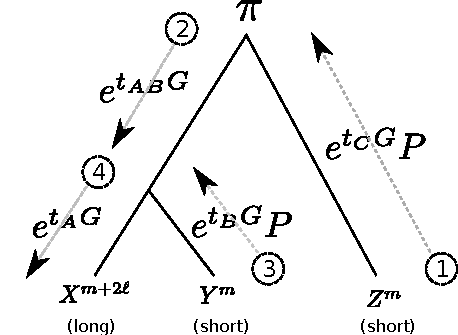
\includegraphics{peeling-schematic}
\end{center}

To compute the likelihood on a more complicated tree, consider the following,
with the three-taxon tree above as an example,
where we are counting occurrences of (long) $m+2\ell$-tuples in taxon $X$,
and (shorter) $m$-tuples in taxa $Y$ and $Z$.

We can compute the likelihood in a similar way, summing over the root state (the summation over $u$)
and the interior node ($v$):
\begin{align} \label{eqn:three_taxa_likelihood}
  \begin{split}
    & \P\{X_{I-\ell}^{m+2\ell}=x \text{ and } Y_I^\ell=y \text{ and } Z_I^\ell=z \} \\
    &\qquad = \sum_{u \in \calS^{m+2\ell}} \pi(u) p_{m,\ell}(t_C,u,z) \sum_{v \in \calS^{m+2\ell}} p_{m+2\ell}(t_{AB},u,v) p_{m+2\ell}(t_{A},v,x) p_{m,\ell}(t_B,v,y)
  \end{split}
\end{align}
The steps for computing this are then:
\begin{enumerate}

  \item Compute $M_1(u,z) = p_{m,\ell}(t_C,u,z)$ (a $|\calS|^{m+2\ell} \times |\calS|^m$ matrix)

  \item Compute $M_2(v,z) = \sum_{u \in \calS^{m+2\ell}}  p_{m+2\ell}(t_{AB},u,v) \pi(u) M_1(u,z)$ (still a $|\calS|^{m+2\ell} \times |\calS|^m$ matrix)

  \item Compute $M_3(v,y) = p_{m,\ell}(t_B,v,y)$ (a $|\calS|^{m+2\ell} \times |\calS|^m$ matrix)

  \item Compute $M_4(x,(y,z)) = \sum_{v \in \calS^{m+2\ell}} p_{m+2\ell}(t_{A},v,x) M_2(v,z) M_3(v,y)$ (stored as a $|\calS|^{m+2\ell} \times |\calS|^{2m}$ matrix).

\end{enumerate}
Then $M_4$ gives all the likelihoods.
This is depicted in the figure, writing $\left(e^{tG}\right)_{ab}$ for the matrix $p_{m+2\ell}(t,a,b)$,
and $P$ for the projection matrix that gives $p_{m,\ell}(t,a,b) = \left( e^{tG} P\right)_{ab}$.


In total there are $|\calS|^{3m+2\ell}$ possible data combinations.
However, we can reduce dimensionality by replacing the last step with
\begin{enumerate}

  \item[4'.] Compute $M_4(x,w) = \sum_{v \in \calS^{m+2\ell}} p_{m+2\ell}(t_{A},v,x) M_3(v,w) M_4(v,w)$ (stored as a $|\calS|^{m+2\ell} \times |\calS|^{m}$ matrix).

\end{enumerate}
and only computing the likelihood for cases with $y=z=w$.
On a three-taxon tree it is not clear that this is desireable, since missing out on double transitions
might be a significant loss of information,
but on larger trees it seems likely that we'd want to restrict to combinations with most sites agreeing across the tree.
(Note, however, that one should not first look at the data, observe which combinations $(y,z)$ were most common, and then restrict to only those!)


\subsection*{Algorithm}

Fix one tip of the tree, $a$, to be the taxa where we count ``long'' sequences, let $\rho$ be the root, and let $b_1, \ldots, b_n$ be the remaining tips,
where we observe ``short'' sequences.
Let $v_0=\rho, v_1, \ldots, v_\ell = a$ be the path from the root down to $a$,
let $u_1, u_2, \ldots, u_m$ be the remaining internal nodes,
and for each $v_i$ let $u(v_i)$ be the offspring of $v_i$ that is not one of the other $v$.
For each node in the tree,
we will compute a matrix of probabilities:
for nodes not on the path from $a$ to the root,
we compute the chance that that each ``long'' sequence observed at that node
is matched by each possible combination of ``short'' sequences on the tips of the tree below it.
For nodes on the path from $a$ to the root, we compute the probability of observing
each ``long'' sequence at that node, along with the combinations of ``short'' sequences
on all tips further away from $a$ (i.e.\ below that node if it was rooted at $a$).
For a node $w$ this will be stored as a $|\calS|^{m+2\ell} \times |\calS|^{cm}$ matrix, for some $c$,
and denoted $M(w)$.
Rows of $M(u_j)$ sum to 1,
while each entire matrix $M(v_i)$ sums to 1;
the difference being that $M(v_i)$ sums over the prior at the root,
and $M(u_j)$ takes the value at $u_j$ as given.

Let $t(w)$ be the length of the branch above node $w$, for $w \neq \rho$,
and denote by $G^T$ the transpose of $G$.

\begin{enumerate}

  \item Set $M(b_i) = P$ for each $b_i$.

  \item While there are $u_j$ whose children $w_1$ and $w_2$ both have matrices computed,
    \begin{enumerate}
      \item let
        \begin{align}
          M(u_j)_{x,(y,z)} = \left( e^{t(w_1) G} M(w_1) \right)_{x,y} \left( e^{t(w_2) G} M(w_2)_{x,z} \right)_{x,z} .
        \end{align}
    \end{enumerate}

  \item Let
    \begin{align}
      M(\rho)_{x,y} = \pi(x) \left( e^{t(u(\rho)) G} M(w(\rho)) \right)_{x,y}
    \end{align}

  \item For each $1 \le k < \ell$,
    \begin{enumerate}
      \item let
        \begin{align}
          M(v_k)_{x,(y,z)} = \left( e^{t(v_k) G^T} M(v_{k-1}) \right)_{y,x} \left( e^{t(u(v_k)) G} M(u(v_{k-1})) \right)_{x,z}  .
        \end{align}
    \end{enumerate}

  \item Finally, let
    \begin{align}
      M(a)_{x,y} = \left( e^{t(a) G^T} M(v_{\ell-1}) \right)_{x,y}  .
    \end{align}

\end{enumerate}



%%%%%%
\section{Bayesian things}

So, suppose we've got a list of patterns $(x_i,y_i)$
and we're happy with the idea that they're independent.
Recall that
\[
\E\left[ N(x,y) \mid N(x) \right] = N(x) p_{m,\ell}(x,y) ,
\]
Parameters $\theta$ enter implicitly through $p_{m,\ell}$.


In the case that we observe the initial sequence, $N(x,y)$ are binomial with sample size $N(x)$.
and so the likelihood is
\[
\prod_x N(x)! \prod_y \frac{ p_{m,\ell}(x,y)^{N(x,y)} }{ N(x,y)! } ,
\]
and so the negative log likelihood is, up to a constant,
\[
\sum_{x,y} N(x,y) \log p_{m,\ell}(x,y) .
\]


%%%%%%
\section{Full likelihood}

\emph{The following is copied over from work on the abphylo project.}

The s5f model is defined as follows:
for each $(a,b,c,d,e,x) \subset \{\nA,\nC,\nG,\nT\}$,
it gives a (relative) mutation rate
\begin{align}
    \gamma(c,x;a,b,d,e) = \text{( mutation rate of $c \to x$ in context $abcde$ )} .
\end{align}
Given these rates, the only unknown parameter is the total amount of time
that the sequence has been mutated for.
Suppose that $X(t)$ is a sequence of length $n$ evolving under this model,
and let $G_n$ be the corresponding generator matrix,
a $4^n \times 4^n$ matrix.
(In the s5f model, the mutation rates are only specified in the middle of 5-mers,
so the two bases on each end never mutate.)
The transition probabilities are $e^{tG_n}$,
and by marginalization,
we can compute quantities like
the probability for observing the middle set of basis
given the flanking $\ell$ on each end:
\begin{align}
    p_{\ell,n-2\ell}(t;a,b)
    &=
    \P\{
        (X_{\ell+1}(t), X_{\ell+2}(t), \ldots, X_{n-\ell}(t))=(b_1,b_2,\ldots,b_{n-2\ell}) \\
    &\qquad \qquad
        \given (X_{1}(0), X_{2}(0), \ldots, X_{n}(0))=(a_1,a_2,\ldots,a_{n})
    \} .
\end{align}
If the size of the context, $\ell$, is big enough,
then this probability will not depend significantly if the sequence $a$ is in fact embedded in a longer sequence
(the error decreases exponentially with $\ell$).

The sequence $X(t)$ can be constructed by beginning with $X(0)$,
putting down a Poisson process of potential mutations of rate $\gamma = \max\{\gamma(c,x;a,b,d,e)\}$,
and thinning appropriately.
The process depends on the flanking 2bp,
so any other mutation within 2bp of a site affects the process at that site,
and the chance that this occurs depends on the flanking 4bp on either side.
Concretely, the number of flanking positions in each direction
that must be kept track of to decide what happens at a given site
grows by 1 at rate $\gamma$, and by 2 at rate $\gamma$;
so the amount of flanking sequence on each side affecting a given site at time $t$
is the sum of a Poisson($\gamma t$) and twice an independent Poisson($\gamma t$).
This has mean $3\gamma t$ and variance $5 \gamma t$;
with high probability it will not exceed, say,
$3\gamma t + 6 \sqrt{\gamma t}$;
if $\gamma t < 1$ this is less than 9.


How can we use this to compute the likelihood of a full sequence?
Actually, we know more.
For two positions $(i,s)$ and $(j,t)$ in sequence $\times$ time,
let $r(i,s;j,t) = |j-i|/|t-s|$ be the slope of the line between them,
and if $I$ and $J$ are subsets of sites, let $r(I,s;J,t) = \min\{r(i,s;j,t) : i\in I, j \in J\}$
be the minimum.
Then, we know that there is a speed of dependency propagation $r_*$
such that if $r(I,s;J,t) > r_*$,
then $X_I(s)$ and $X_J(t)$ are nearly independent.
Now, fix $t$ and for each site $i$ let $N_i$ denote its $r_*$-neighborhood,
i.e.,
\begin{align}
    N_i = \{ (j,s) : r(i,t; j,s) \le r_*, \; 0 \le s \le t \} .
\end{align}
These are depicted in figure~\ref{fig:neighborhoods}A.
We will write $i \sim j$ if $|i-j| \le 2 r_* t$,
or equivalently, if $N_i \cap N_j \neq \emptyset$,
and $i \nsim j$ otherwise.
We can think of $N_i$ as the parts of ancestral sequences in which a mutation might have affected the state at $(i,t)$.
so if $i \nsim j$, then $i$ and $j$ are (approximately) independent at time $t$, given the sequence at time 0.
Concretely,
we have a small $\epsilon$ such that for any $i \nsim j$,
\begin{align}
    &\big|
    \log( \P\{ X_i(t) = x_i \and X_j(t) = x_j \} ) \\
    &\qquad {} -
    \log( \P\{ X_i(t) = x_i \} \P\{ X_j(t) = x_j \} )
    ) \big|
    \le \epsilon .
\end{align}


\begin{figure}
    \begin{center}
        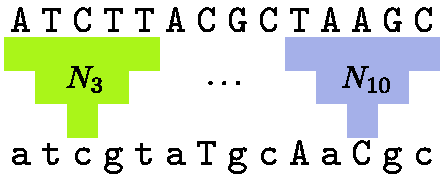
\includegraphics{context-neighborhoods-defns}

        \vspace{2em}

        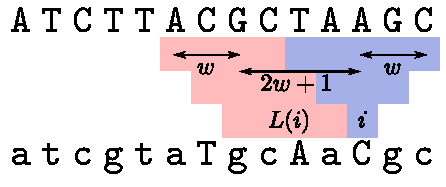
\includegraphics{context-neighborhoods-widths}
    \end{center}
    \caption{
        Diagram of things in the text:
        (top) Dependency neighboorhods.
        (bottom) What we need to compute $\P\{X_i(t)=x \given X(0), X_{<i}(t)\}$:
        site $i$ depends on the blue squares in $N_i$;
        the sites to the left of this in $L(i)$ are those other sites in $X(t)$
        whose dependency neighborhoods overlap $N_i$;
        any further sites to the left of this are basically independent of $X_i(t)$;
        the red squares give the dependency neighborhood of $L(i)$,
        so we need to condition on the row of red and blue sites at the top.
        On the bottom, we have $2w+1$ sites; at the top we have $4w+1$;
        here $w=2$.
        \label{fig:neighborhoods}
    }
\end{figure}



What we'd like to know is the likelihood, i.e.,
\begin{align}
    \like(y|x)
    &:=
    \P\{ X(t) = y \given X(0) = x \} .
\end{align}
If we define $X_{<i}=(X_1, \ldots, X_{i-1})$, then
\begin{align}
    \like(y|x)
    &=
    \prod_{i=1}^n
    \P\{ X_i(t) = y_i \given X(0) = x \and X_{<i}(t) = y_{<i} \} .
\end{align}
Now, defining $L(i) = \{ j < i \st j \sim i \}$
to be the sites to the left of $i$ whose dependency neighborhoods overlap with $i$'s,
and $A(I) = \{ j \st |j-i| \le r_*t \text{ for some } i \in I\}$
to be the ancestral sites in the dependency neighborhood of $I$,
\begin{align}
&\big|
\log( \P\{ X_i(t) = y_i \given X(0) = x \and X_{<i}(t) = y_{<i} \} ) \\
& \qquad {} -
\log( \P\{ X_i(t) = y_i \given X_{A(L(i))}(0) = x_{A(L(i))} \and X_{L(i)}(t) = y_{L(i)} \} )
 \big| \\
&\qquad \qquad \le
    \epsilon ,
\end{align}
so that if we define
\begin{align}
    \alike(y|x)
    &=
    \prod_{i=1}^n
    \P\{ X_i(t) = y_i \given X_{A(L(i))}(0) = x_{A(L(i))} \and X_{L(i)}(t) = y_{L(i)} \} ,
\end{align}
then (with $\loglike = \log \like$),
\begin{align}
    \left| \aloglike(y|x) - \loglike(y|x) \right|
    \le n \epsilon .
\end{align}

This is good, because we can compute $\aloglike$:
let $w=r_*t$ be radius of a dependency neighborhood,
so that the width of $L(i)$ is $2w$,
and for a sequence $x$ define $x^{(m)}_i = (x_{i-m+1}, \ldots, x_i)$:
\begin{align}
    \alike(y|x)
    &=
    \prod_{i=1}^n
    \frac{
        p_{w,2w+1}(y^{(2w+1)}_i|x^{(4w+1)}_{i+w})
    }{
        p_{w,2w}(y^{(2w)}_{i-1}|x^{(4w)}_{i-1+w})
    }
\end{align}
This is the ratio of the likelihoods of all the $(w,2w+1)$ T-mers,
divided by the likelihoods of all the $(w,2w)$ T-mers.




%%%%%%%
\section{Simulation results}

The method works well to find point estimates of the parameters.
Obtaining posterior density estimates using the approximation likelihood function on a subset of patterns
works in some cases;
in other cases the likelihood surface is still too peaked, underestimating the uncertainty.

\subsection{TASEP}

Strings of length $10^5$ were evolved under TASEP for varying amounts of time,
and pattern occurrences counted.
Running 10,000 MCMC iterations with window sizes of $\ell=w=3$ (total length 9) on these takes around 40 minutes.
Apparently, the patterns used were not sufficiently independent in this case,
as the posterior is too sharp.

Here's a short example sequence with $\lambda=1$:
\begin{center}
 \setlength{\tabcolsep}{0pt}
\begin{tabular}{cccccccccccccccccccccccccccccccccccccccccccccccccccccccccccc}
X&X&X&O&O&X&O&O&O&O&X&O&X&O&X&X&O&O&X&O&O&X&O&X&X&X&O&X&O&O&O&X&X&O&X&O&O&O&X&X&O&O&O&X&O&O&O&O&X&O&X&X&O&X&X&O&O&X&O&O \\
$\centerdot$&O&X&O&X&O&O&O&X&$\centerdot$&O&X&O&O&X&X&X&o&x&$\centerdot$&o&O&X&x&x&O&X&O&X&o&o&O&X&X&$\centerdot$&$\centerdot$&o&o&O&X&X&o&$\centerdot$&O&X&$\centerdot$&o&o&$\centerdot$&$\centerdot$&O&X&X&x&O&X&o&O&X&$\centerdot$
\end{tabular}
\end{center}
here particles are X's, moving to the right; and spaces are O's;
in the second line,
$\centerdot$ is a position that has not considered a change; lowercase letters are positions that considered a change but did not;
and upper case are positions that did change.

\begin{figure}
  \begin{center}
    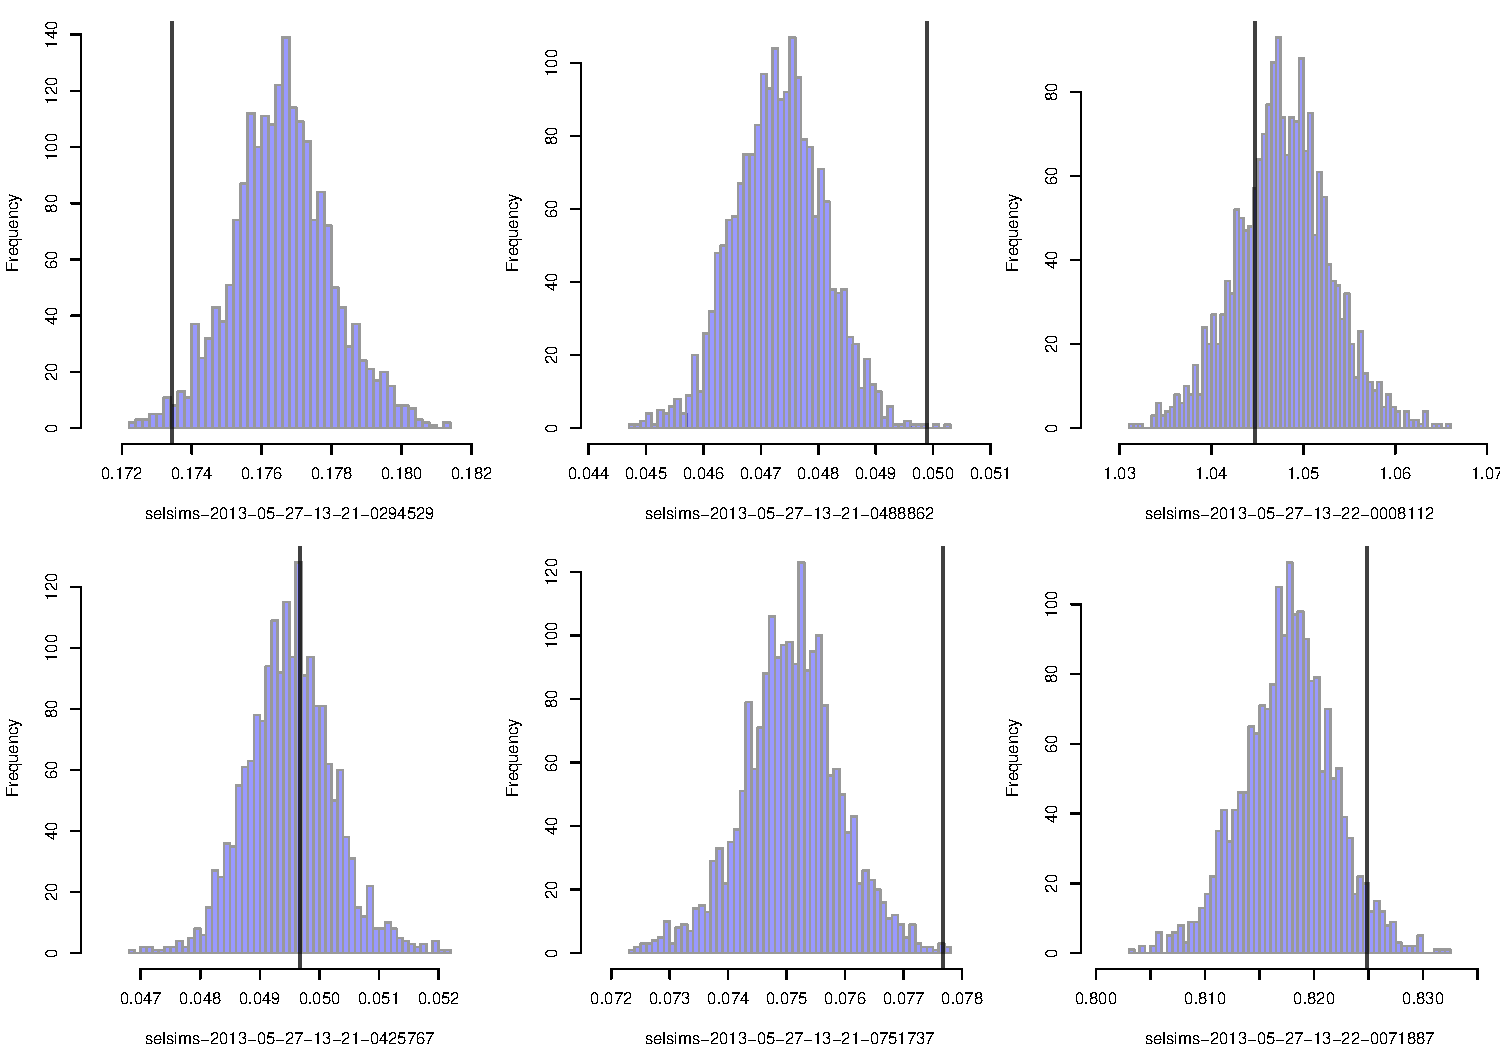
\includegraphics[width=\textwidth]{../tasep/all-mcmc-runs}
  \end{center}
  \caption{ Results from MCMC estimates for six different data sets of the parameter in TASEP (mutation rate multiplied by time).
  Vertical line shows the true value.
  }
\end{figure}


\subsection{Ising model}

Strings of length $10^6$ were evolved under Glauber dynamics on the Ising model with varying parameters,
and pattern occurrences counted.
As for TASEP, running 10,000 MCMC iterations with window sizes of $\ell=w=3$ (total length 9) on these takes around 40 minutes.
In this case, the true parameter values have good distribution within the estimated posterior distributions.

Here is an example, with all parameters equal to 1, for $t=.5$:
\begin{center}
 \setlength{\tabcolsep}{0pt}
\begin{tabular}{cccccccccccccccccccccccccccccccccccccccccccccccccccccccccccc}
X&X&O&X&X&O&O&X&O&X&O&X&X&O&O&X&O&O&O&O&X&X&X&O&X&O&X&O&X&O&O&O&X&X&O&X&X&X&X&X&O&X&O&X&O&X&X&X&X&O&O&X&X&X&X&X&X&O&O&O \\
x&x&o&x&X&X&O&x&o&x&$\centerdot$&x&x&O&X&X&$\centerdot$&O&X&O&X&x&x&o&x&o&x&o&x&O&X&O&$\centerdot$&$\centerdot$&O&O&X&X&O&X&X&X&o&x&o&$\centerdot$&X&O&X&o&o&x&X&X&X&O&X&o&$\centerdot$&$\centerdot$
\end{tabular}
\end{center}
The notation is as above; except that the entire matched pattern involved in a change is uppercase:
to simulate, we look in windows of size 3; so if XOO changes to XXO, the whole thing is uppercase, not just the middle X.

\begin{figure}
  \begin{center}
    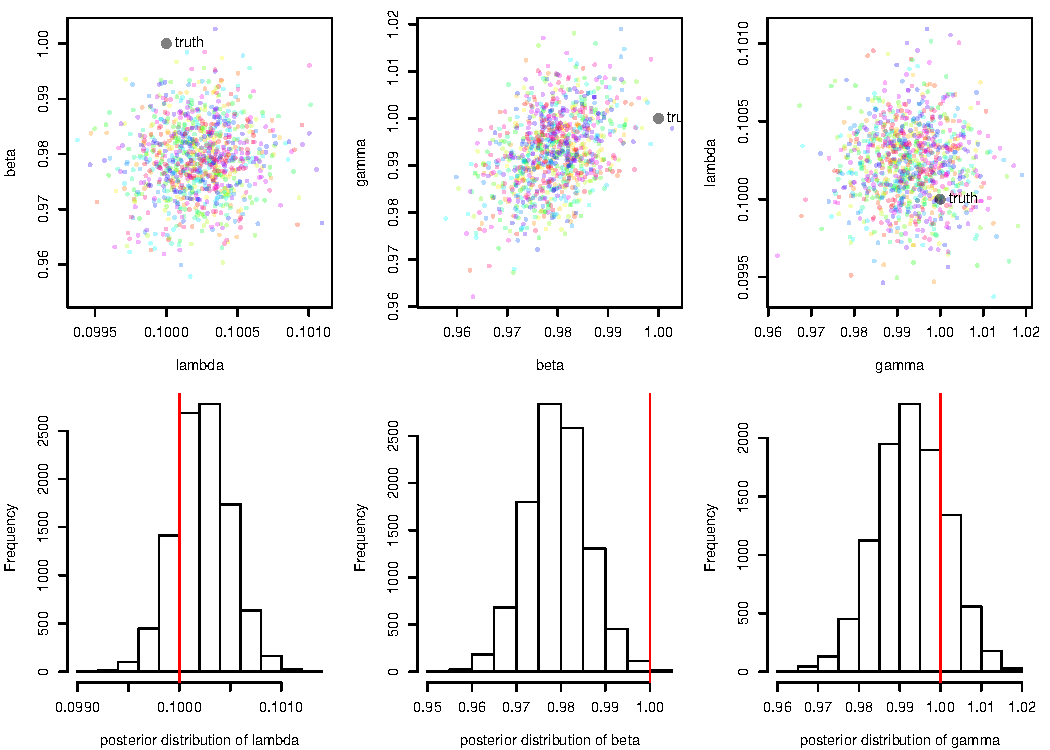
\includegraphics{writeup-plots/selsims-2013-05-28-17-12-0275615-traces}
  \end{center}
  \caption{
  MCMC traces of the parameters in the Ising model across 100,000 iterations.
  The units of $\lambda$ are in mean number of changes per site.
  Vertical line shows the true value.
  }
\end{figure}

\begin{figure}
  \begin{center}
    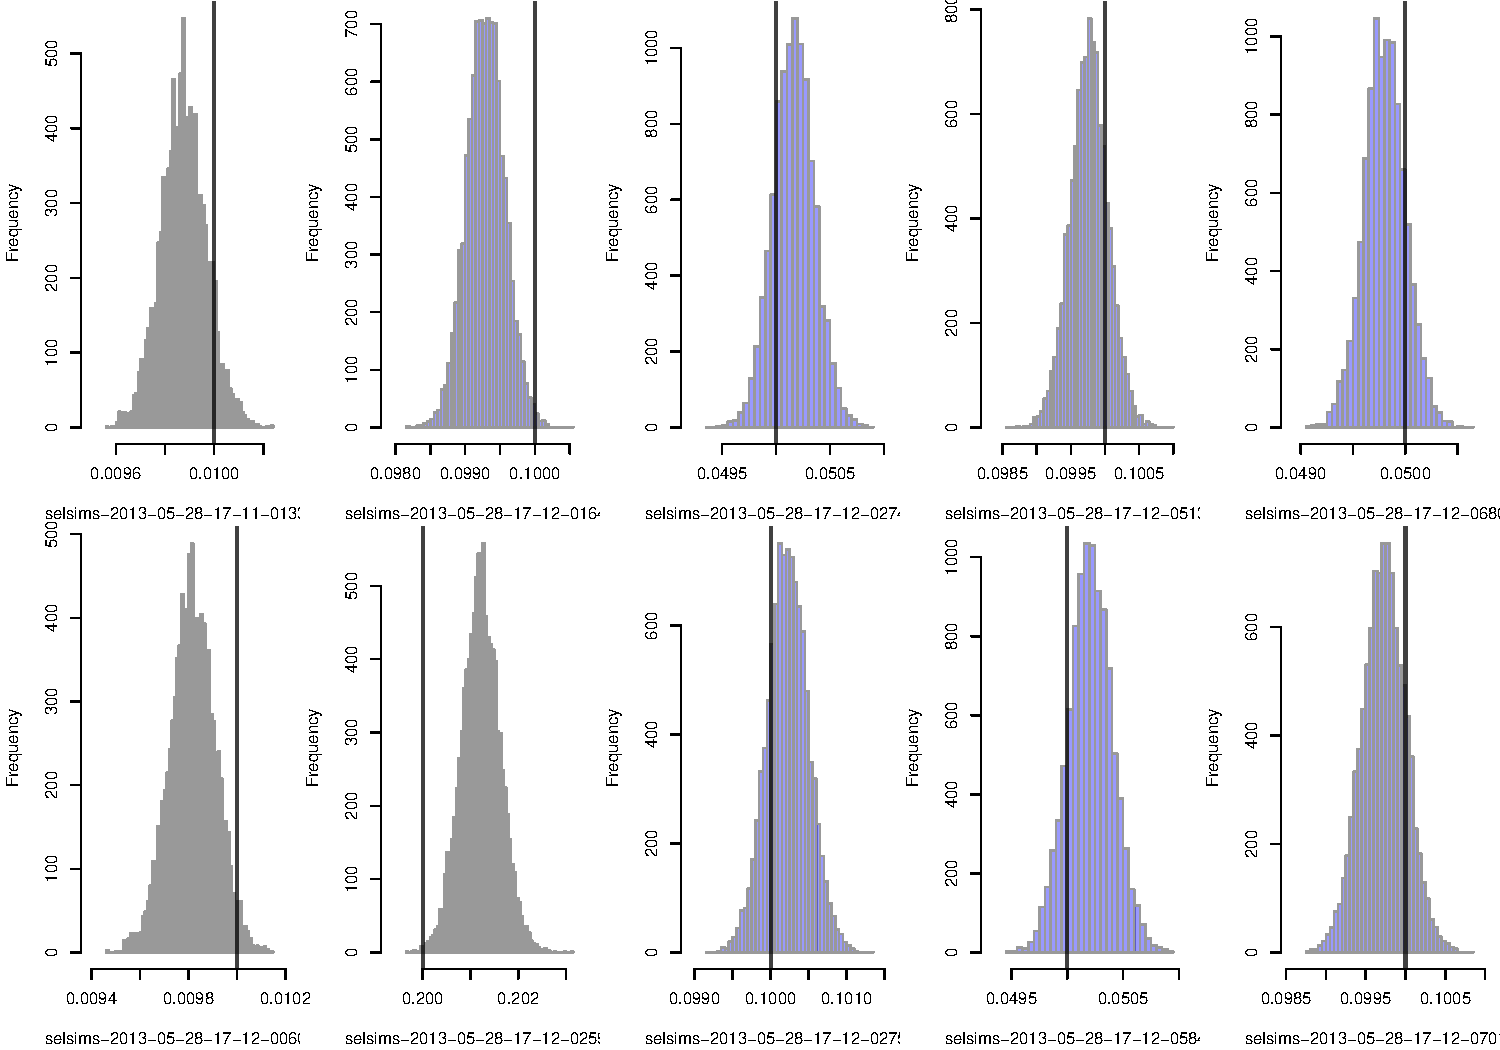
\includegraphics[width=\textwidth,page=1]{../ising/all-mcmc-runs}
  \end{center}
  \caption{ Results from MCMC estimates of the time-scaled mutation rate parameter $\lambda t$,
  in ten different simulated datasets under the Ising model.
  Vertical line shows the true value.
  }
\end{figure}

\begin{figure}
  \begin{center}
    \includegraphics[width=\textwidth,page=2]{../ising/all-mcmc-runs}
  \end{center}
  \caption{ Results from MCMC estimates of the inverse temperature $\beta$ in the Ising model.
  Vertical line shows the true value.
  }
\end{figure}

\begin{figure}
  \begin{center}
    \includegraphics[width=\textwidth,page=3]{../ising/all-mcmc-runs}
  \end{center}
  \caption{ Results from MCMC estimates of the magnetization parameter $\beta$ in the Ising model.
  Vertical line shows the true value.
  }
\end{figure}

%%%
\subsection{CpG mutation, on a tree}

Nucleotide sequences of length $10^6$ were simulated down two (unequal) branches of a tree,
with all single-base substitution rates $m_{xy}$ set equal (varying from a total of .01 to .1 across the tree)
and an additional CpG rate $\gamma$ set to either 0 or three times the single-base rate.
Analysis was done with $\ell=2$ and $w=1$ (a five-to-one window).

The state at the root of the tree was independently chosen bases with equal frequencies,
and these frequencies at the root were added as parameters to the model (with a Dirichlet prior).

Here is a short example, with all parameters equal to 1, with each branch of the tree having length $0.1$:
\begin{center}
 \setlength{\tabcolsep}{0pt}
\begin{tabular}{cccccccccccccccccccccccccccccccccccccccccccccccccccccccccccc}
T&G&G&A&G&A&G&G&T&C&T&G&C&C&A&T&A&G&A&C&G&G&G&C&G&C&C&G&C&C&T&A&G&G&A&G&C&C&G&C&G&T&T&T&T&G&C&G&T&G&G&T&G&T&T&G&T&G&G&C \\
$\centerdot$&$\centerdot$&g&C&G&a&$\centerdot$&$\centerdot$&$\centerdot$&$\centerdot$&T&A&C&A&$\centerdot$&$\centerdot$&$\centerdot$&T&A&T&$\centerdot$&$\centerdot$&$\centerdot$&T&G&c&C&C&A&C&$\centerdot$&$\centerdot$&$\centerdot$&$\centerdot$&$\centerdot$&$\centerdot$&$\centerdot$&$\centerdot$&$\centerdot$&G&G&G&t&A&T&$\centerdot$&$\centerdot$&G&A&g&C&G&$\centerdot$&$\centerdot$&$\centerdot$&$\centerdot$&t&T&G&A \\
$\centerdot$&$\centerdot$&$\centerdot$&$\centerdot$&$\centerdot$&$\centerdot$&$\centerdot$&A&T&$\centerdot$&$\centerdot$&$\centerdot$&$\centerdot$&$\centerdot$&$\centerdot$&T&T&G&T&$\centerdot$&$\centerdot$&G&A&T&$\centerdot$&$\centerdot$&$\centerdot$&G&G&c&t&A&A&G&C&$\centerdot$&$\centerdot$&$\centerdot$&G&T&G&A&t&t&t&g&$\centerdot$&$\centerdot$&$\centerdot$&$\centerdot$&$\centerdot$&$\centerdot$&G&A&$\centerdot$&$\centerdot$&$\centerdot$&$\centerdot$&A&C
\end{tabular}
\end{center}
Top is ancestral sequence (``unobserved''); bottom two are at the tips.

The point estimates are good,
as are the MCMC estimates,
but there seems to be mixing trouble having to do with the root frequencies.

\begin{figure}
  \begin{center}
    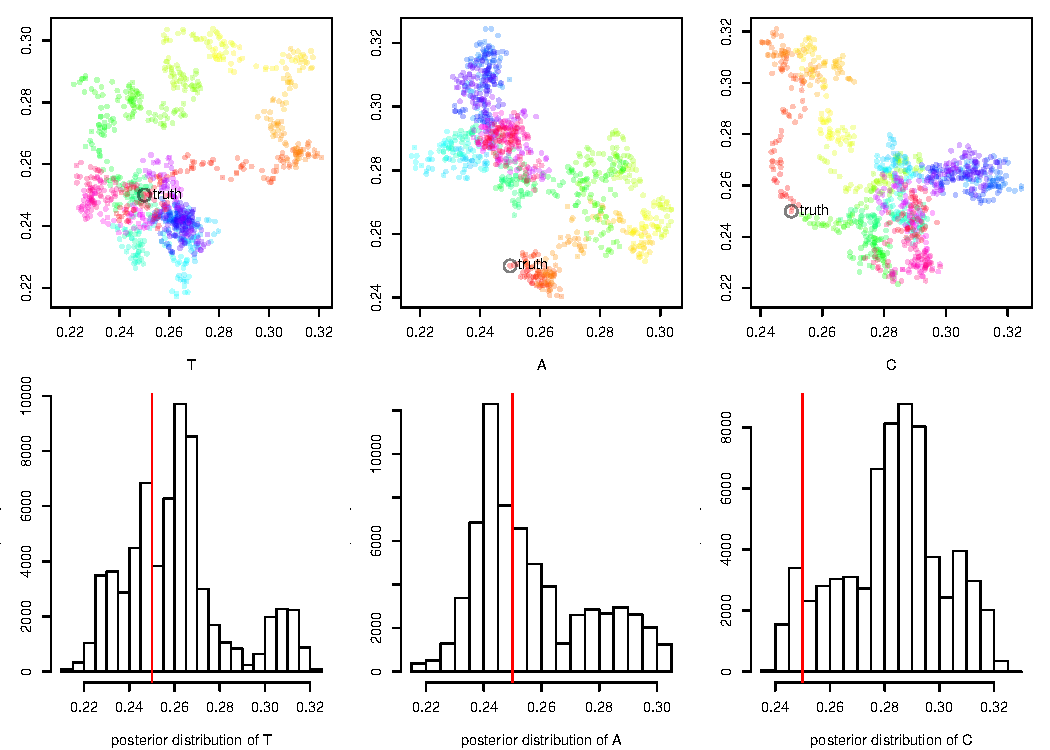
\includegraphics{writeup-plots/selsims-2013-06-03-13-17-0790276-initfreqs}
  \end{center}
  \caption{
  MCMC traces across 660,000 iterations of the frequencies at the root of the (two-taxon) tree in the CpG model.
  Vertical line shows the true value.
  }
\end{figure}

\begin{figure}
  \begin{center}
    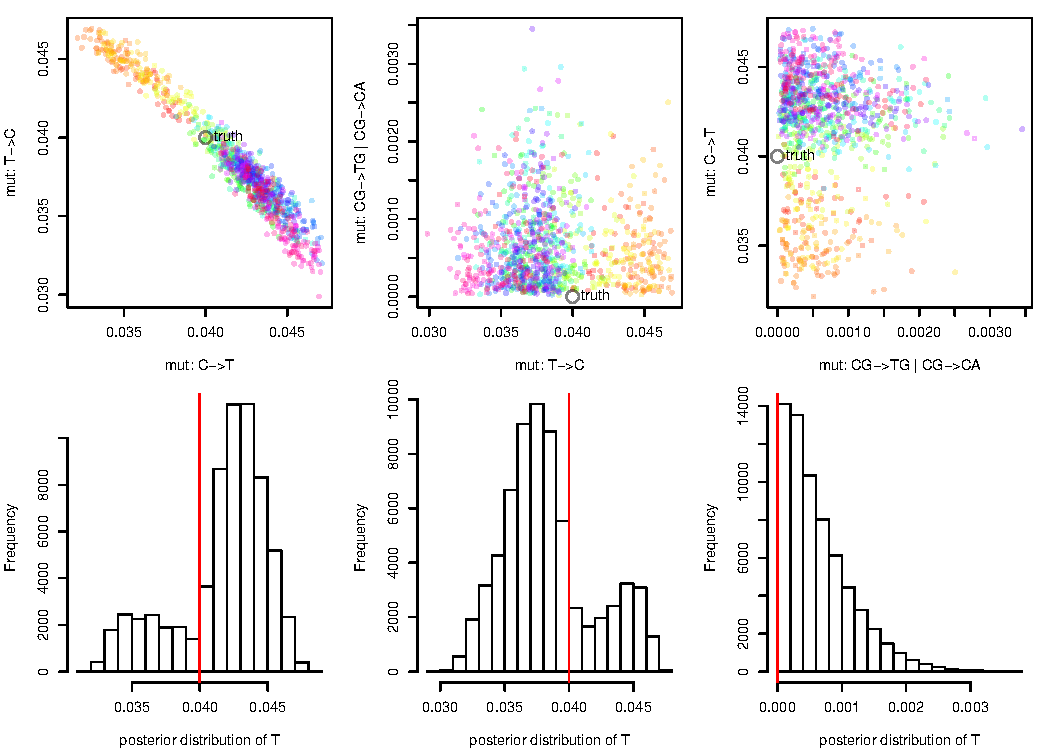
\includegraphics{writeup-plots/selsims-2013-06-03-13-17-0790276-mutrates}
  \end{center}
  \caption{
  MCMC traces across 660,000 iterations of several mutation rate parameters in the CpG model.
  Units are in mean number of substitutions per base across the entire tree.
  Vertical line shows the true value.
  }
\end{figure}

%%%%%%%%
\section{Power sims}

Assess power and accuracy in the Ising model, by running replicates at these parameters:

\begin{tabular}{|rlllrrr|}
  \hline
  seqlen   &  $\lambda t$   &  $\beta$  &  $\gamma$  &  $w$ &  $\ell$   & \# reps \\
  \hline
  $10^4$    &   .2  &   1   &   .5  &   3   &   3   &   10  \\
  $10^3$    &   .2  &   1   &   .5  &   3   &   3   &   10  \\
  $10^2$    &   .2  &   1   &   .5  &   3   &   3   &   10  \\
  \hline
  $10^4$    &   .4  &   1   &   .5  &   3   &   3   &   10  \\
  $10^4$    &   .1  &   1   &   .5  &   3   &   3   &   10  \\
  $10^4$    &   .05  &   1   &   .5  &   3   &   3   &   10  \\
  \hline
  $10^4$    &   .2  &   1   &   0  &   3   &   3   &   10  \\
  \hline
  $10^4$    &   .2  &   1   &   .5  &   3   &   2   &   10  \\
  $10^4$    &   .2  &   1   &   .5  &   3   &   1   &   10  \\
  $10^4$    &   .2  &   1   &   .5  &   3   &   0   &   10  \\
  \hline
\end{tabular}

\section{Applications}

graham:
\begin{itemize}

\item estimating freq spectrum [Hernandez]

\item probabilistic ancestral states for common ancestor of e.g. humans 4N generations ago [Siepel] -- would widely used for primates

\end{itemize}


sergey:
\begin{itemize}

  \item ancestral CpG

  \item ancient DNA

\end{itemize}


%%%%%%%%
\section{What next}

\begin{enumerate}

  \item Allow more than single-base distribution at the root.

  \item What's up with the mixing problem in root frequencies?

  \item See if counting in nonoverlapping windows fixes the peakiness problem with TASEP. \emph{Yes, it does.}

  \item See what's feasible with a larger alphabet -- 60 codons -- and more parameters.

  \item Show that taking no context ($\ell=0$) can be positively misleading in some context.

  \item Do a three-taxa tree.

  \item How to identify motifs in the residuals?

\end{enumerate}

\bibliography{context-dependence}

\end{document}
